%%This is a very basic article template.
%%There is just one section and two subsections.
\documentclass[times,10pt,twocolumn,letterpaper]{article}
\usepackage{ncvpripg}
\usepackage{times}
\usepackage[pdftex]{graphicx}	
\usepackage[cmex10]{amsmath}
\usepackage{url}

\title{Stagnant Water Detection Using quadcopter}
\author{}
\def\iccvPaperID{0000}
\begin{document}
\maketitle

\begin{abstract}
Recently, in urban areas there has been a sharp increase in dengue and malaria.
One of the major reason for this is suspected to be the amount of stagnant
water around residencies. There are many areas around urban residential places
such as terraces of high rise buildings, and shades above windows
(popularly known as `chhajja') that are hard to reach and hence to inspect. We
use quadcopter to inspect such areas and detect whether there is stagnant water.

\end{abstract}

\section{Introduction}

\subsection{Significance of problem}
\cite{NVBDP_Malaria} \cite{WHO15Malaria} \cite{Cecilia14}  \cite{NVBDP_Dengue}
\cite{WHO15Dengue}

\begin{figure}[h!]
\centering
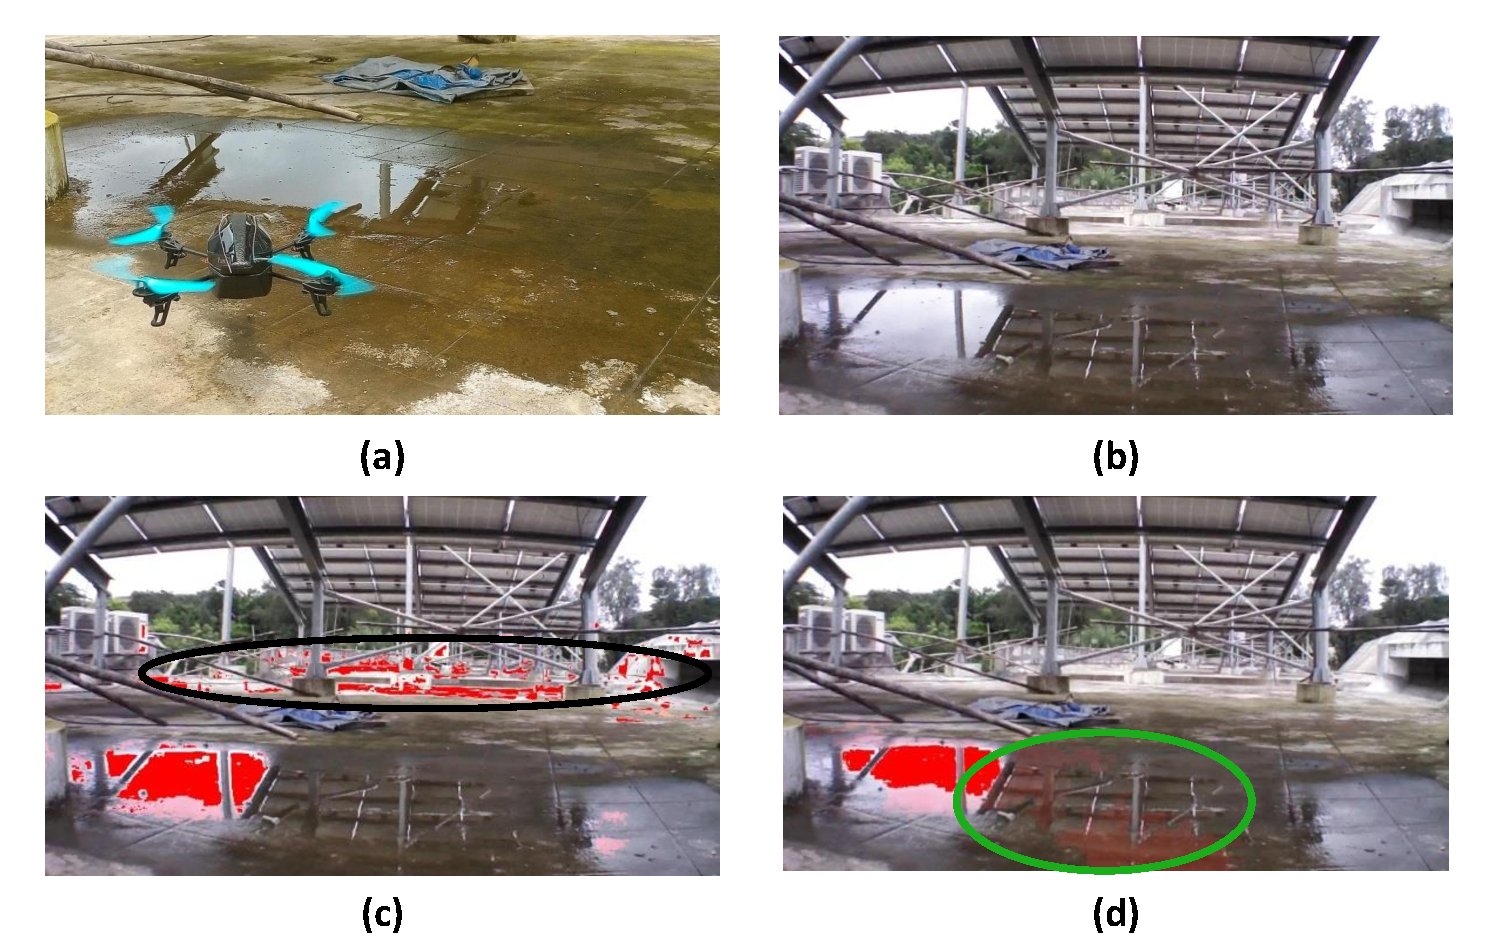
\includegraphics[width=\linewidth]{images/teaser.pdf}
\caption{(a) Quadcopter hovering over stagnant water amassed at building
backyard. (b) Scene captured by quadcopter (c) Our algorithm is able to detect
puddle region in the scene (shown in red).}
\end{figure}

\cite{Microsoft15}

\section{Related Work}

\cite{rankin11}\cite{santana12}\cite{zhang10}

\section{Methodology}

\subsection{SVM classifier}


\begin{figure}[h!]
\centering
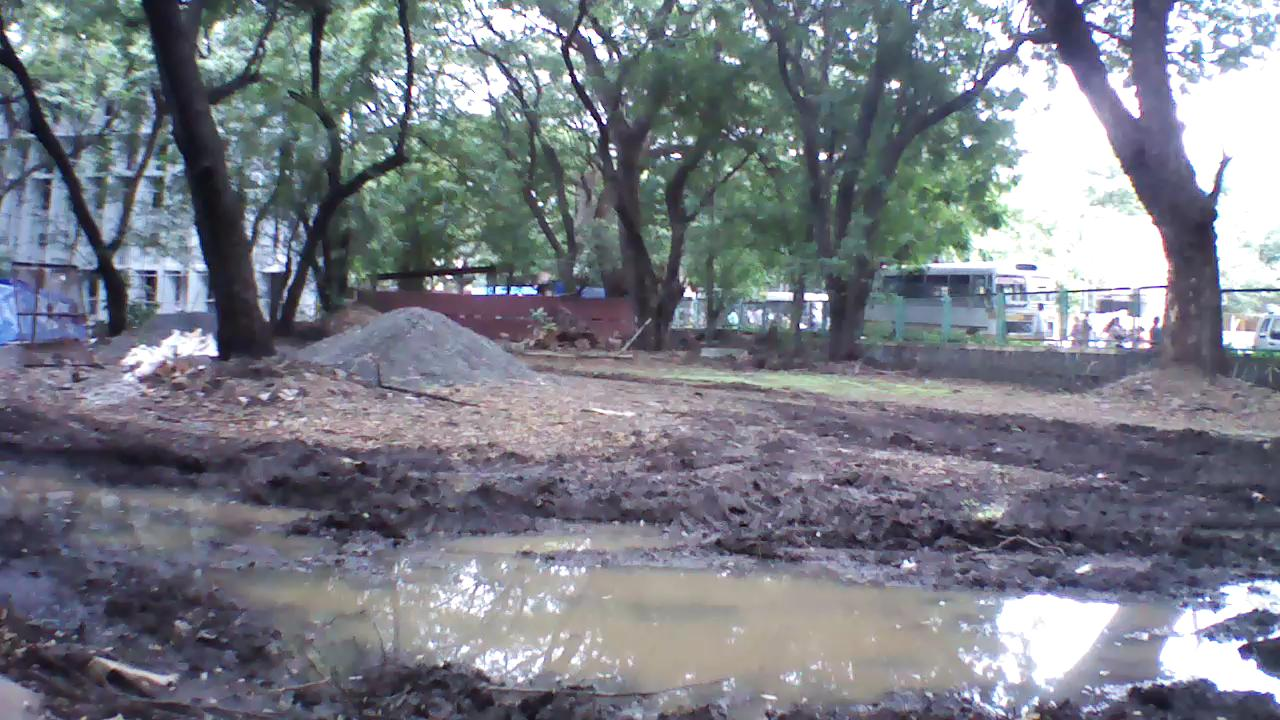
\includegraphics[width=0.22\linewidth]{images/IMG_PAIR_1_1.jpg}
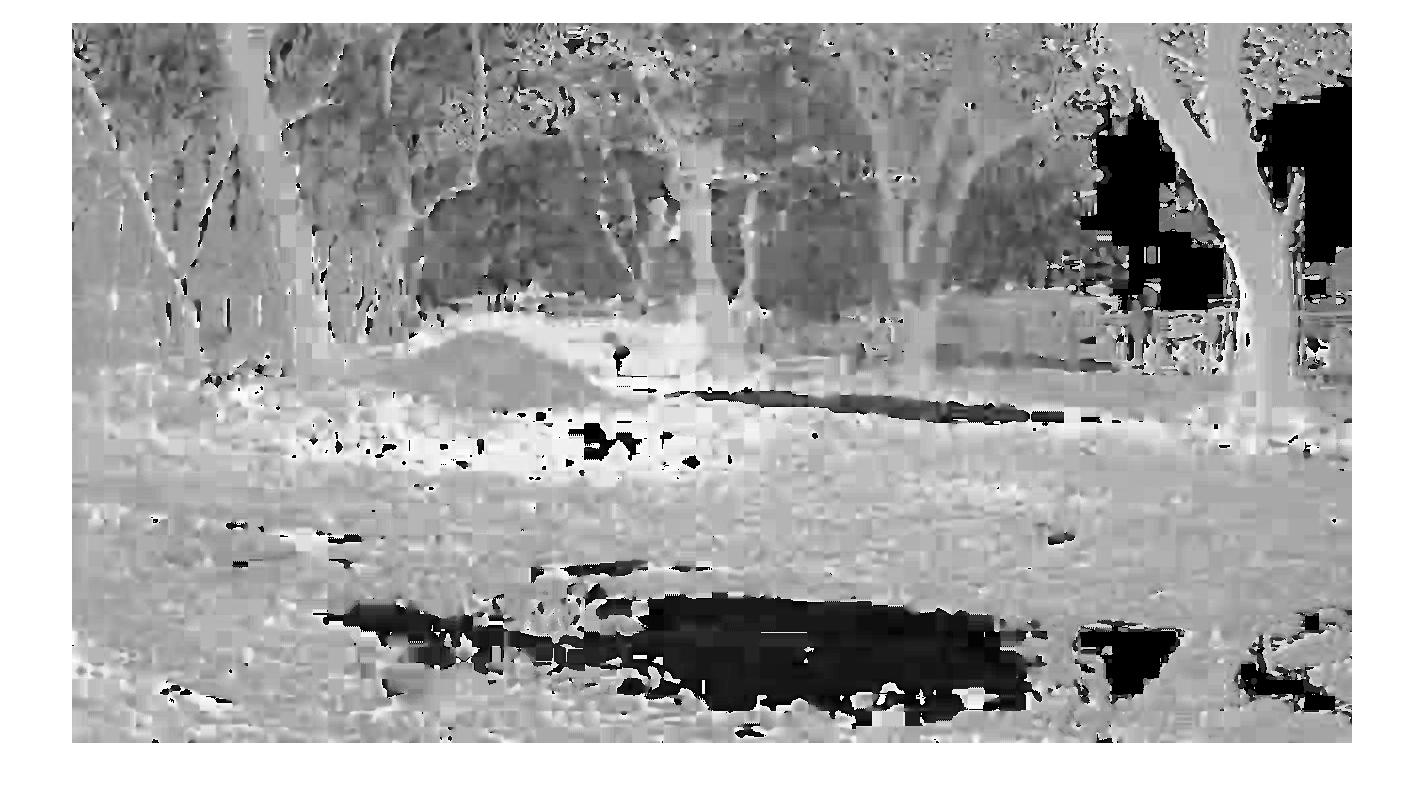
\includegraphics[width=0.22\linewidth]{images/IMG_PAIR_1_1_H.jpg}
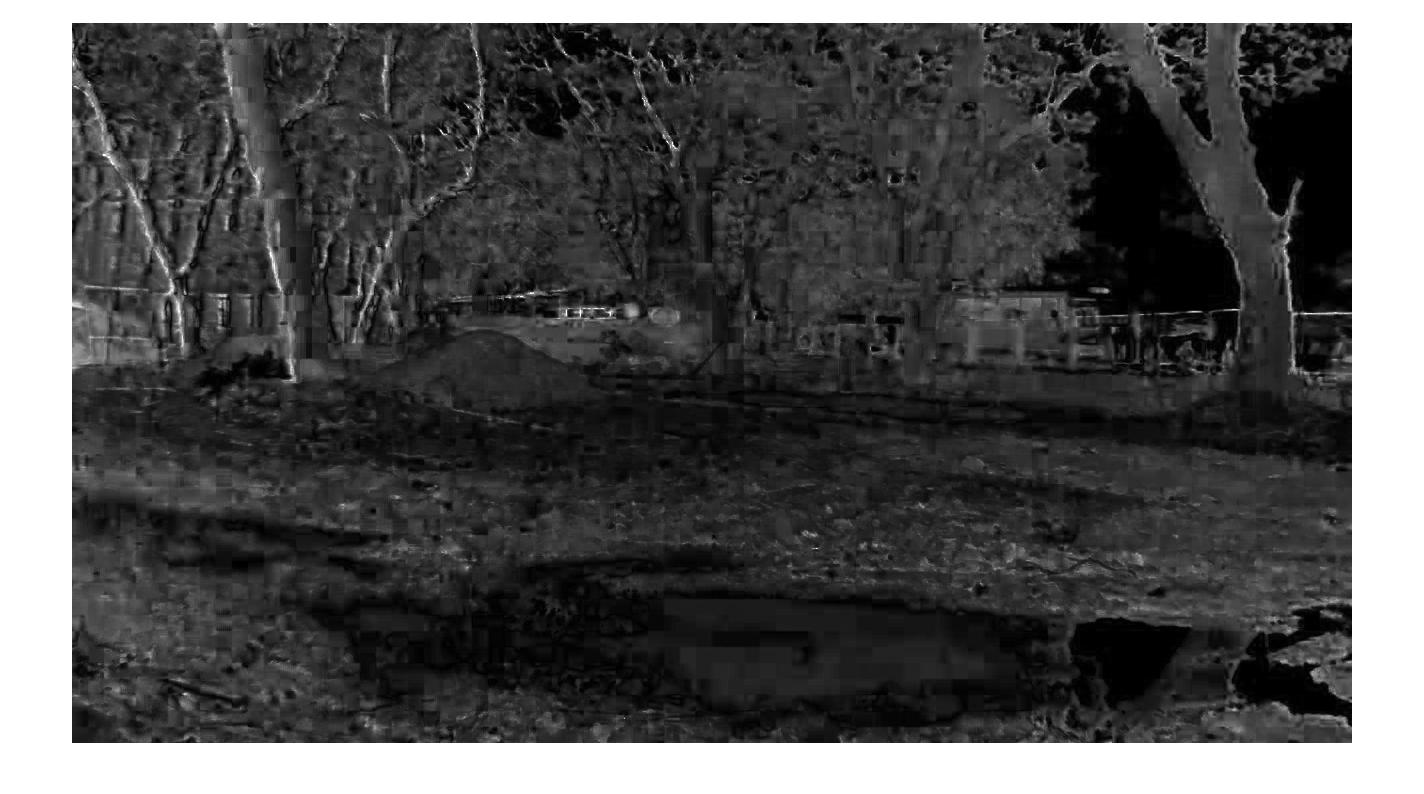
\includegraphics[width=0.22\linewidth]{images/IMG_PAIR_1_1_S.jpg}
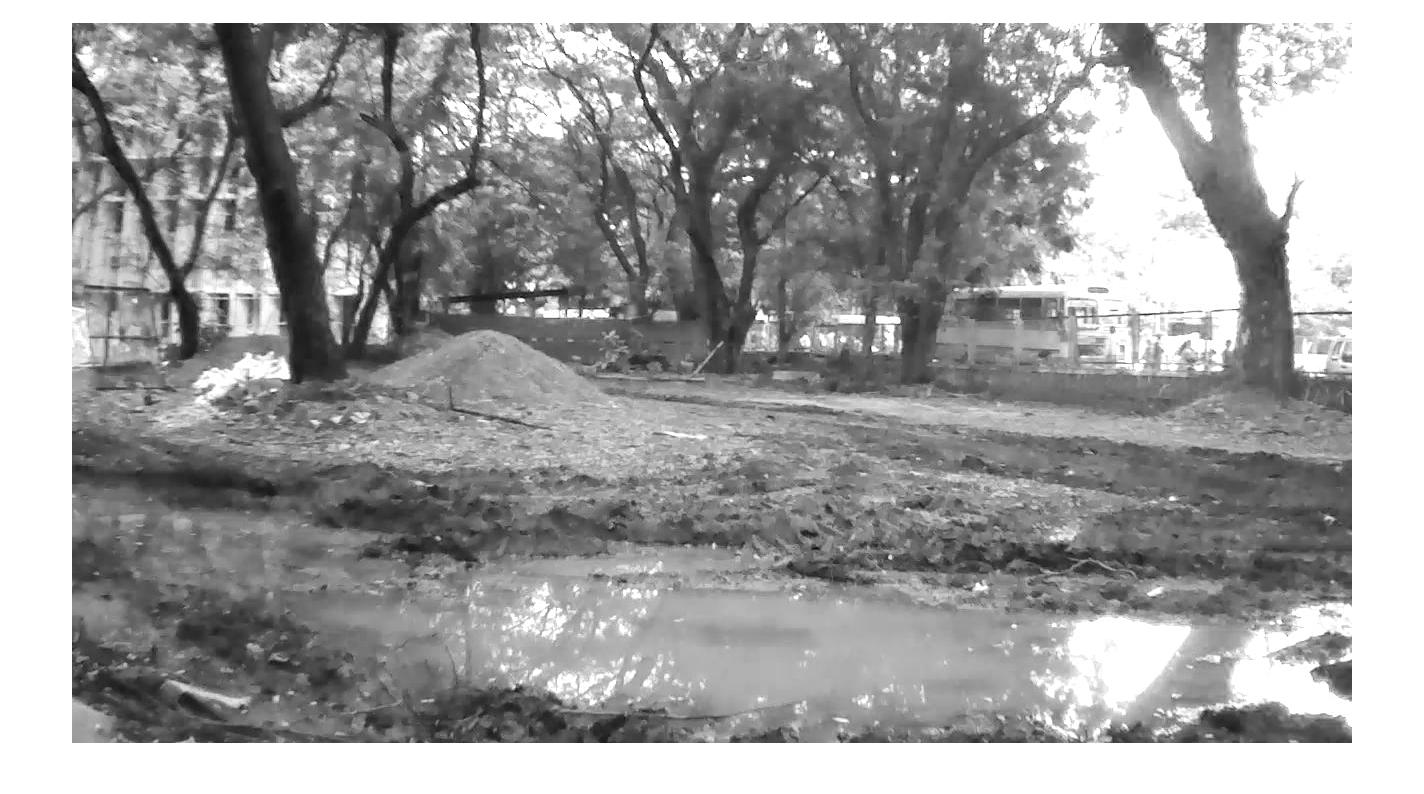
\includegraphics[width=0.22\linewidth]{images/IMG_PAIR_1_1_V.jpg}
\caption{Sample image and their Hue (H), Saturation (S) and Value (V) components
respectively. It can be seen that puddle area has very less Hue as well
as Saturation. Also, reflective parts of puddle has high intensity.}
\label{fig:HSV}
\end{figure}

\cite{Chapelle99}

\subsection{Optical flow based technique}
\begin{figure}[h!]
\centering
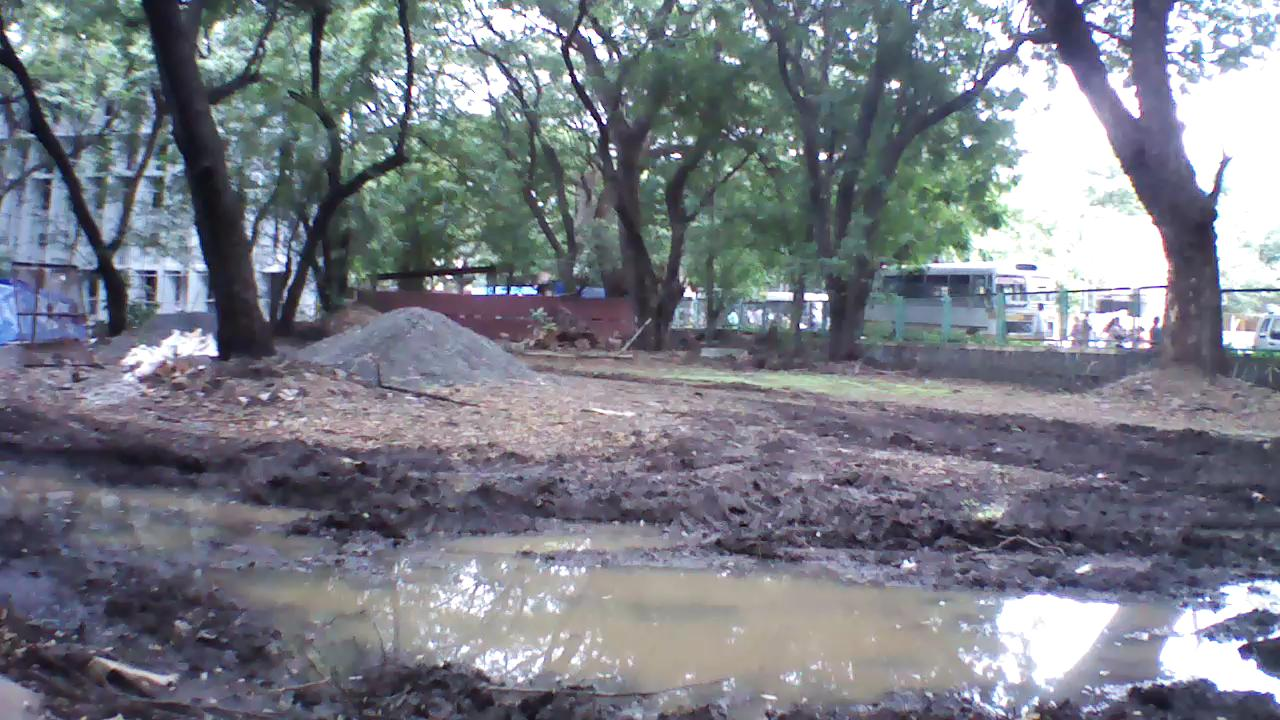
\includegraphics[width=0.3\linewidth]{images/IMG_PAIR_1_1.jpg}
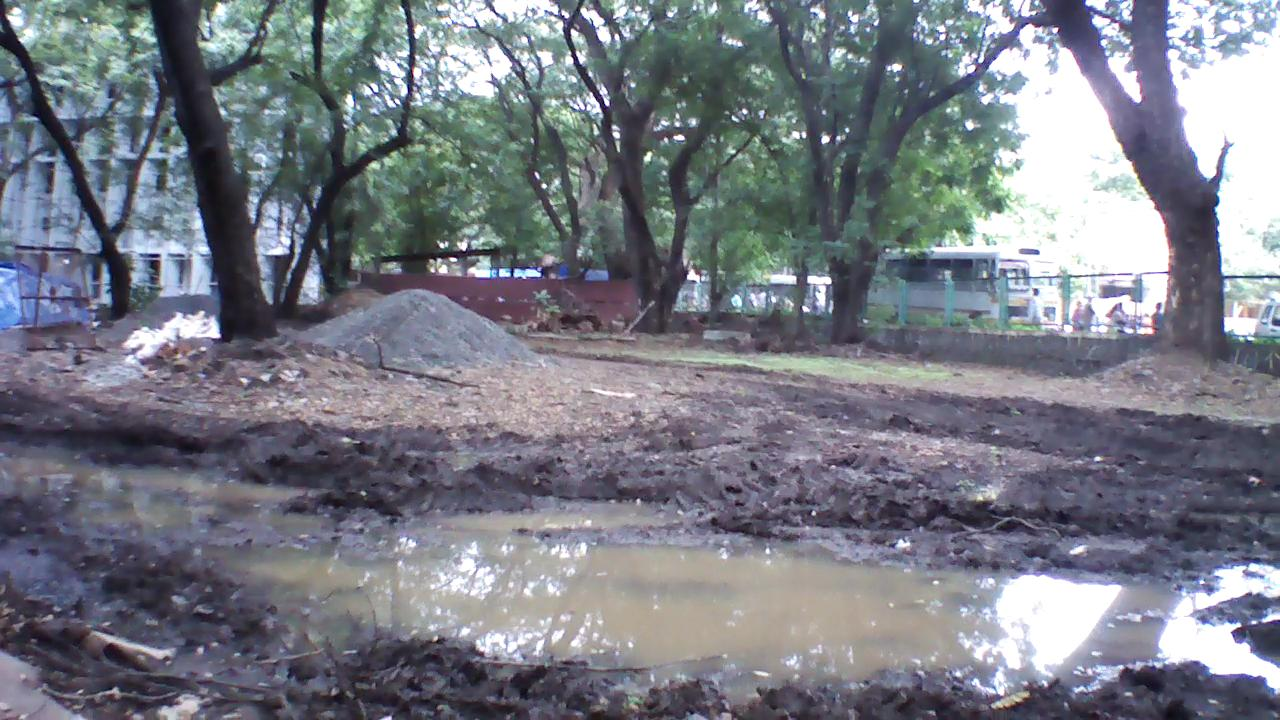
\includegraphics[width=0.3\linewidth]{images/IMG_PAIR_1_2.jpg}
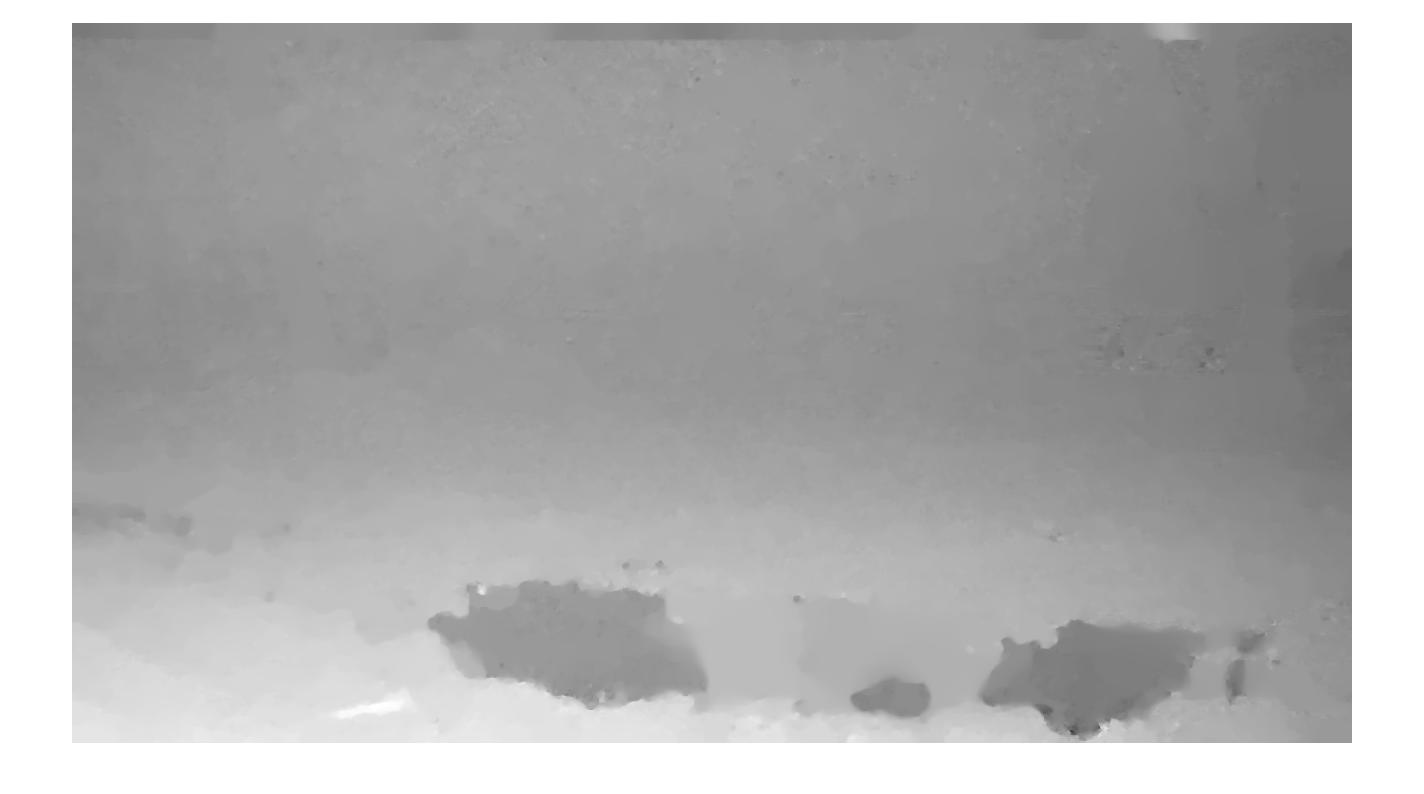
\includegraphics[width=0.3\linewidth]{images/optical_flow_magnitude.jpg}
\caption{Optical Flow. Left, middle: video frames taken from positions
which are $d$ units apart in 3D world. $ 0.01 \leq d \leq 0.1$. Right:
Magnitude of optical flow calculated from earlier images. Magnitude of optical
flow in the reflected parts of the puddle is low compared to that of its
suroundings.}
\end{figure}
\cite{Liu11Thesis}


\cite{Liu11} 
\subsection{Combined approach}

\section{Experiments and Results}
\subsection{Datasets}
\subsection{Creation of training Data}

\begin{figure}[h!]
\centering
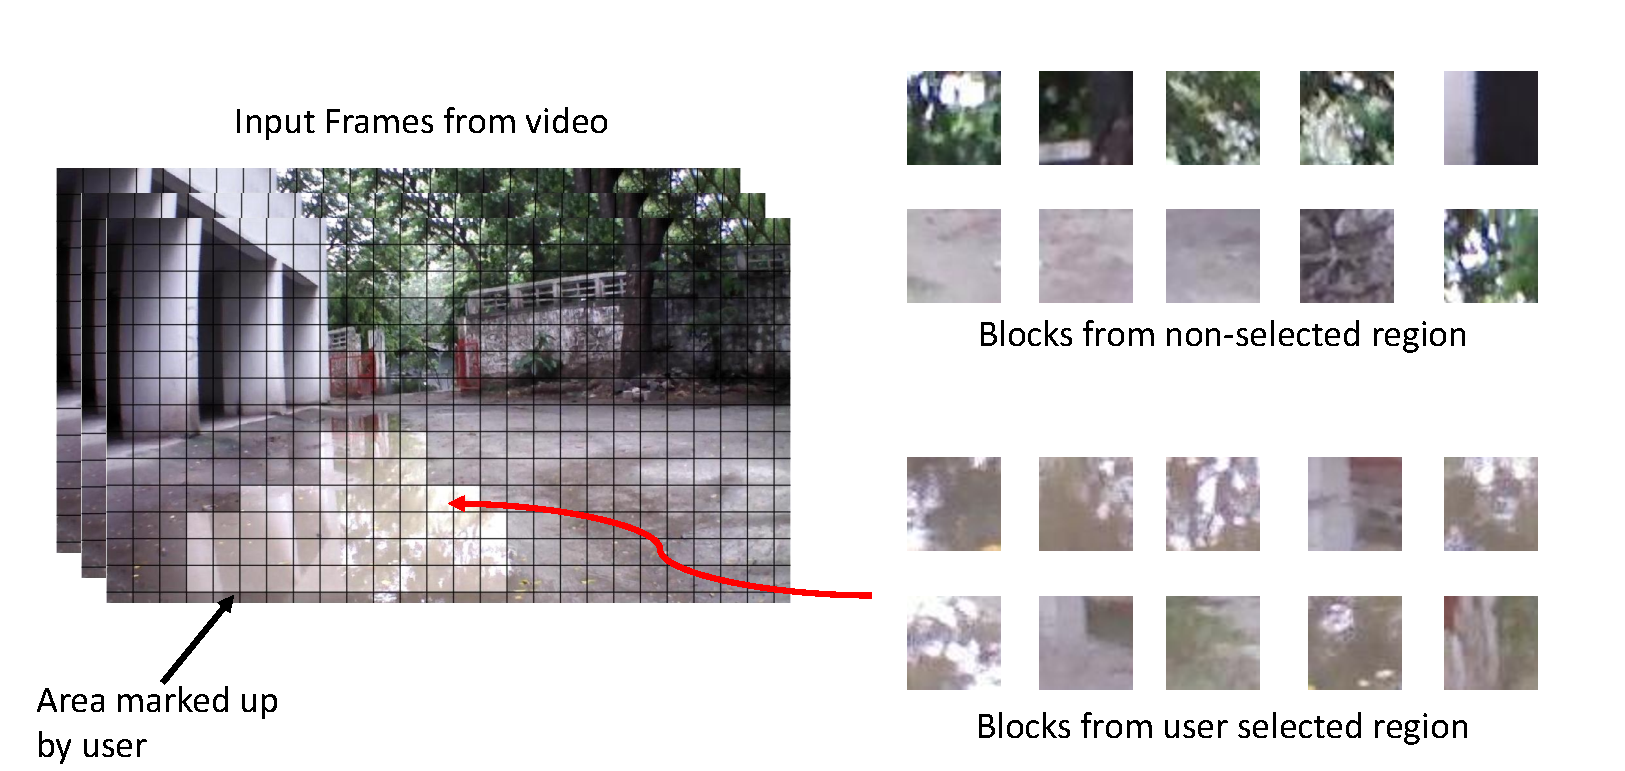
\includegraphics[width=\linewidth]{images/trainingData.pdf}
\caption{Process for creation of training data. User selects puddle area by
drawing a contour over input frame (using our tool). User can additionally
select/deselect blocks which he/she thinks are belonging to puddle/non-puddle
area. We use blocks covered by user drawn contour as `positive' training data.
While the `negative' training data is selected from blocks which are far from
the user drawn contour.}
\label{fig:training}
\end{figure}

\subsection{Comparison with prior technique}
\subsection{Quantitative analysis}
\section{Comclusion and Future Work}

\bibliographystyle{IEEEtran}
\bibliography{egbib}
\end{document}
